\documentclass[11pt,a4paper]{report}
\usepackage[textwidth=37em,vmargin=30mm]{geometry}
\usepackage{calc,xunicode,amsmath,amssymb,paralist,enumitem,tabu,booktabs,datetime2,xeCJK,xeCJKfntef,listings}
\usepackage{tocloft,fancyhdr,tcolorbox,xcolor,graphicx,eso-pic,xltxtra,xelatexemoji}

\newcommand{\envyear}[0]{2025}
\newcommand{\envdatestr}[0]{2025-02-04}
\newcommand{\envfinaldir}[0]{webdb/2025/20250204/final}

\usepackage[hidelinks]{hyperref}
\hypersetup{
    colorlinks=false,
    pdfpagemode=FullScreen,
    pdftitle={Web Digest - \envdatestr}
}

\setlength{\cftbeforechapskip}{10pt}
\renewcommand{\cftchapfont}{\rmfamily\bfseries\large\raggedright}
\setlength{\cftbeforesecskip}{2pt}
\renewcommand{\cftsecfont}{\sffamily\small\raggedright}

\setdefaultleftmargin{2em}{2em}{1em}{1em}{1em}{1em}

\usepackage{xeCJK,xeCJKfntef}
\xeCJKsetup{PunctStyle=plain,RubberPunctSkip=false,CJKglue=\strut\hskip 0pt plus 0.1em minus 0.05em,CJKecglue=\strut\hskip 0.22em plus 0.2em}
\XeTeXlinebreaklocale "zh"
\XeTeXlinebreakskip = 0pt


\setmainfont{Brygada 1918}
\setromanfont{Brygada 1918}
\setsansfont{IBM Plex Sans}
\setmonofont{JetBrains Mono NL}
\setCJKmainfont{Noto Serif CJK SC}
\setCJKromanfont{Noto Serif CJK SC}
\setCJKsansfont{Noto Sans CJK SC}
\setCJKmonofont{Noto Sans CJK SC}

\setlength{\parindent}{0pt}
\setlength{\parskip}{8pt}
\linespread{1.15}

\lstset{
	basicstyle=\ttfamily\footnotesize,
	numbersep=5pt,
	backgroundcolor=\color{black!5},
	showspaces=false,
	showstringspaces=false,
	showtabs=false,
	tabsize=2,
	captionpos=b,
	breaklines=true,
	breakatwhitespace=true,
	breakautoindent=true,
	linewidth=\textwidth
}






\newcommand{\coverpic}[2]{
    % argv: itemurl, authorname
    Cover photo by #2~~(\href{#1}{#1})
}
\newcommand{\makeheader}[0]{
    \begin{titlepage}
        % \newgeometry{hmargin=15mm,tmargin=21mm,bmargin=12mm}
        \begin{center}
            
            \rmfamily\scshape
            \fontspec{BaskervilleF}
            \fontspec{Old Standard}
            \fontsize{59pt}{70pt}\selectfont
            WEB\hfill DIGEST
            
            \vfill
            % \vskip 30pt
            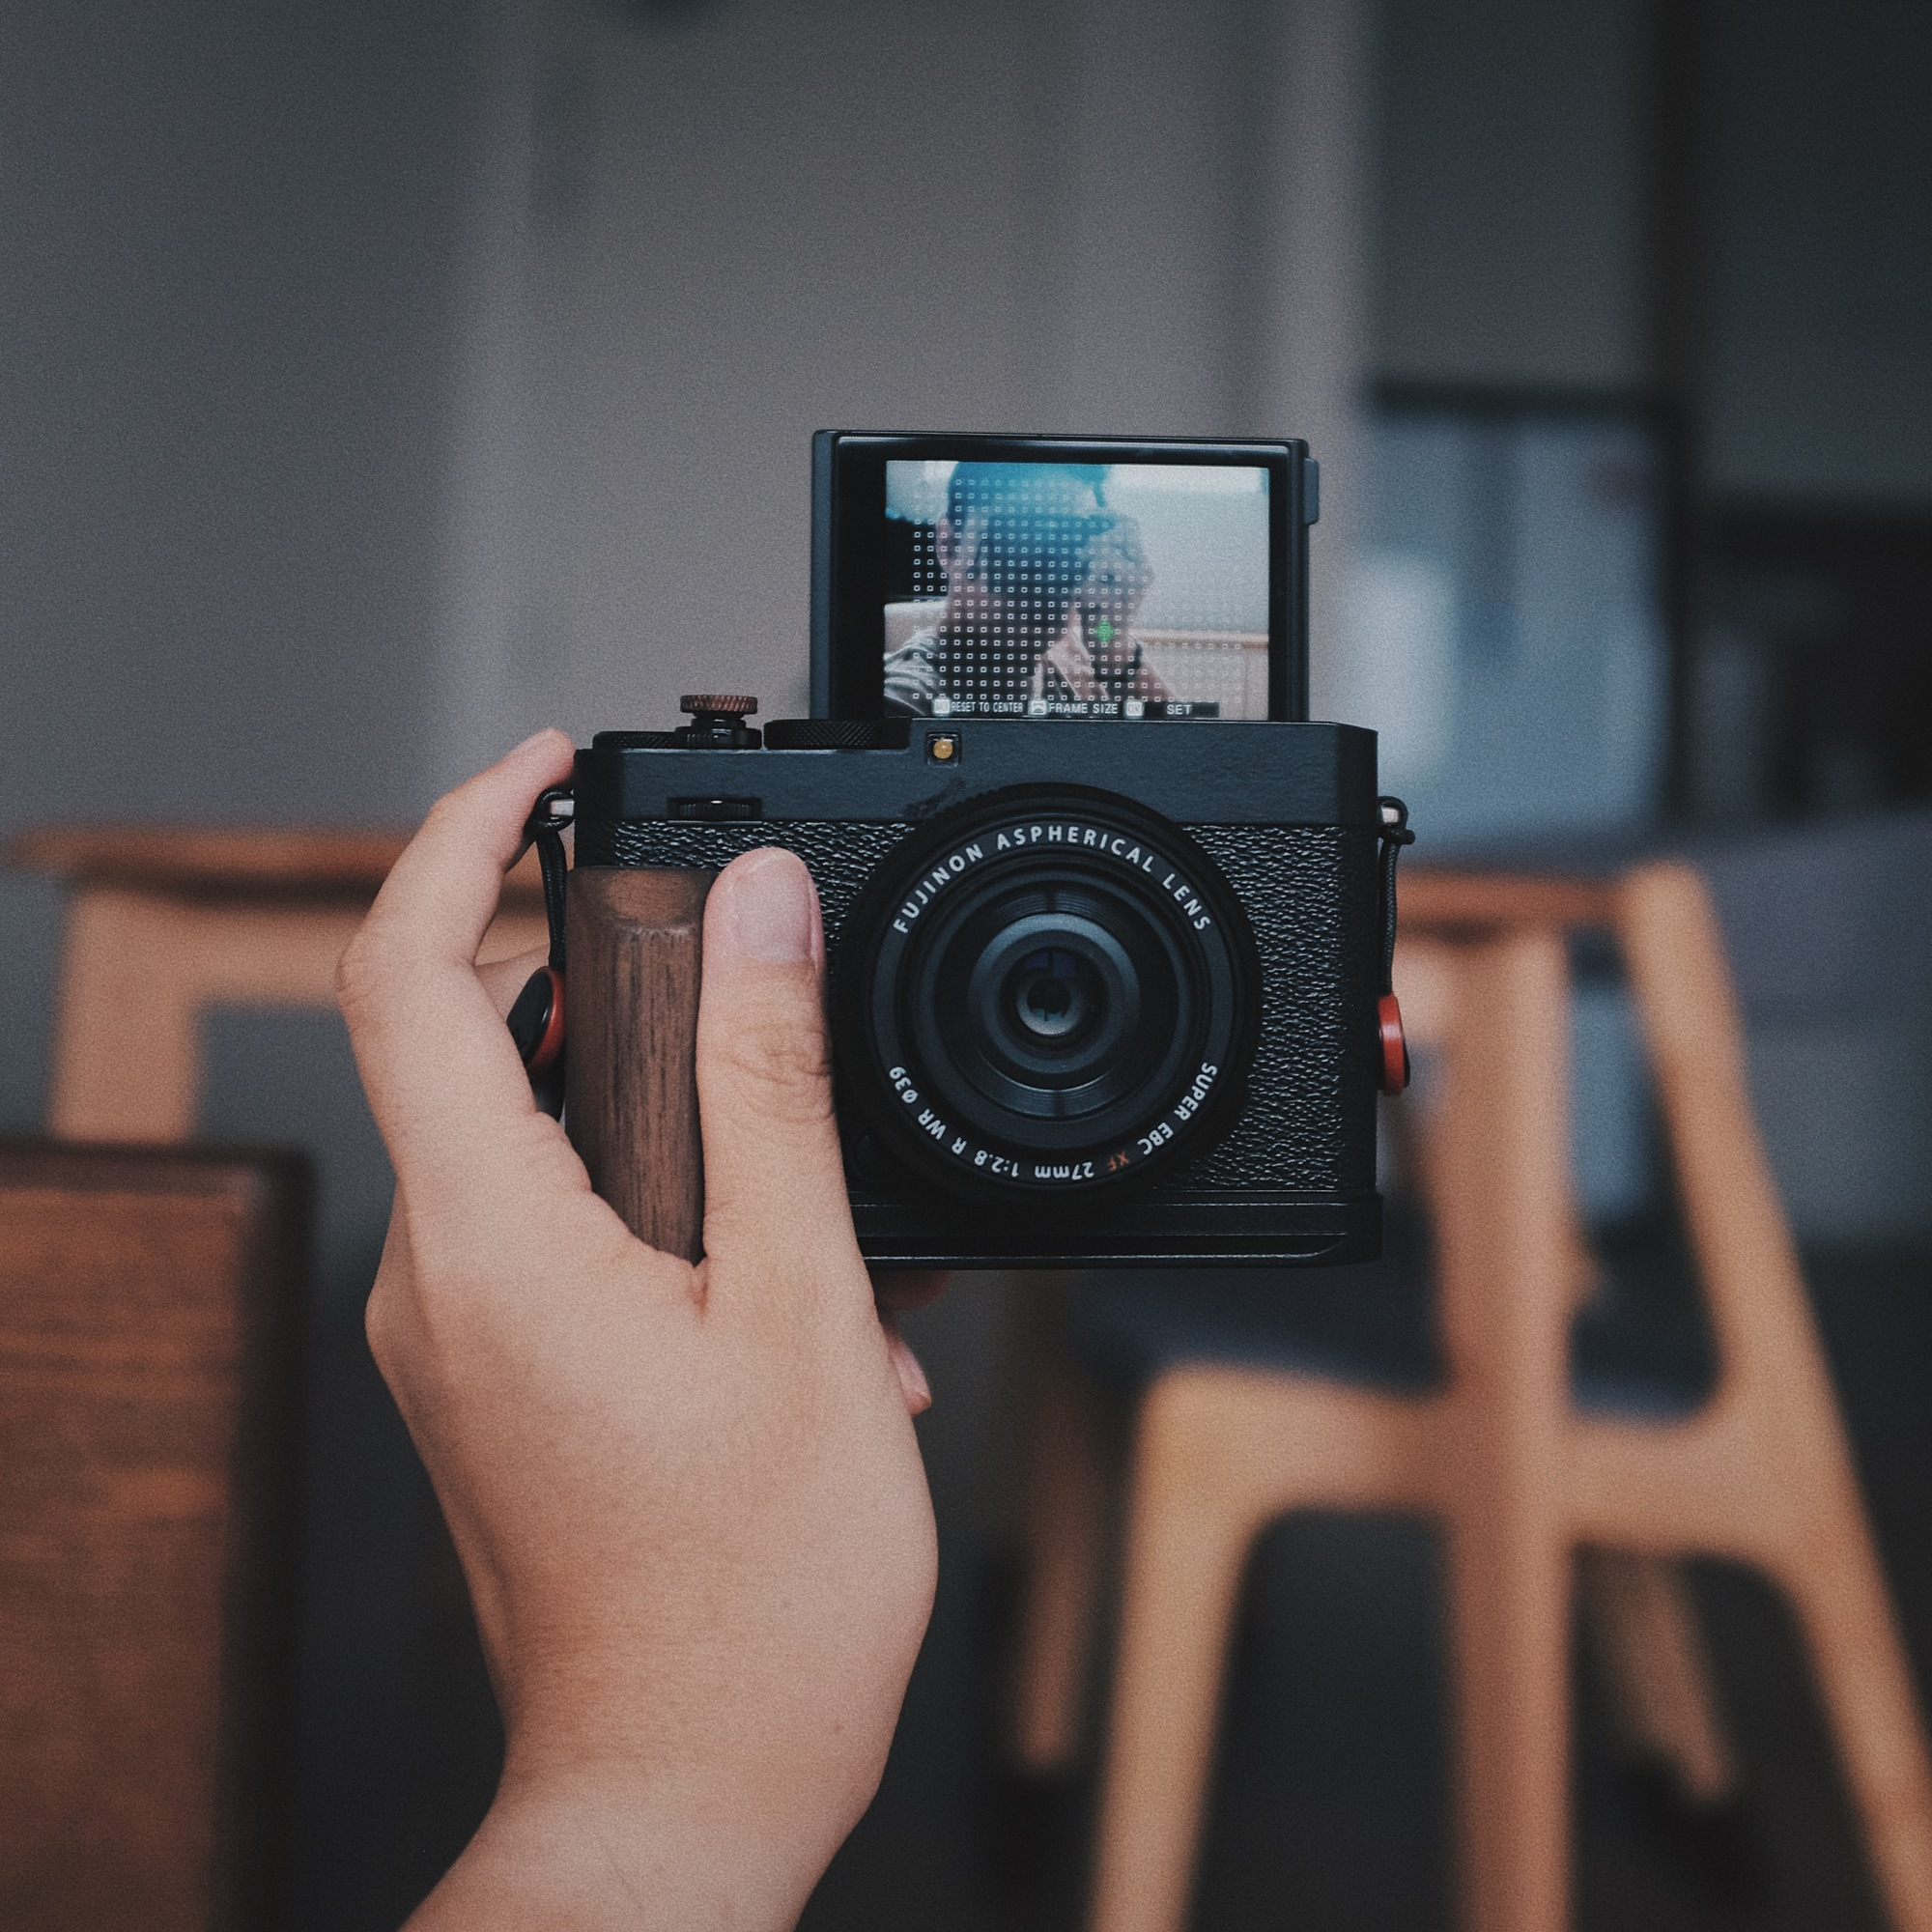
\includegraphics[width=\linewidth]{\envfinaldir/coverpic-prod.jpg}\par
            % \vskip 30pt
            \vfill

            \normalsize\rmfamily\scshape
            \copyright{} The Web Digest Project \hfill\large \envdatestr
        \end{center}
    \end{titlepage}
    % \restoregeometry
}
\newcommand{\simplehref}[1]{%
    \textcolor{blue!80!green}{\href{#1}{#1}}%
}
\renewcommand{\contentsname}{\center\Huge\sffamily\bfseries Contents\par\vskip 20pt}
\newcounter{ipartcounter}
\setcounter{ipartcounter}{0}
\newcommand{\ipart}[1]{
    % \vskip 20pt
    \clearpage
    \stepcounter{ipartcounter}
    \phantomsection
    \addcontentsline{toc}{chapter}{#1}
    % \begin{center}
    %     \Huge
    %     \sffamily\bfseries
    %     #1
    % \end{center}
    % \vskip 20pt plus 7pt
}
\newcounter{ichaptercounter}
\setcounter{ichaptercounter}{0}
\newcommand{\ichapter}[1]{
    % \vskip 20pt
    \clearpage
    \stepcounter{ichaptercounter}
    \phantomsection
    \addcontentsline{toc}{section}{\numberline{\arabic{ichaptercounter}}#1}
    \begin{center}
        \Huge
        \sffamily\bfseries
        #1
    \end{center}
    \vskip 20pt plus 7pt
}
\newcommand{\entrytitlefont}[1]{\subsection*{\raggedright\Large\sffamily\bfseries#1}}
\newcommand{\entryitemGeneric}[2]{
    % argv: title, url
    \parbox{\linewidth}{
        \entrytitlefont{#1}\par\vskip 5pt
        \footnotesize\ttfamily\mdseries
        \simplehref{#2}
    }\vskip 11pt plus 11pt minus 1pt
}
\newcommand{\entryitemGithub}[3]{
    % argv: title, url, desc
    \parbox{\linewidth}{
        \entrytitlefont{#1}\par\vskip 5pt
        \footnotesize\ttfamily\mdseries
        \simplehref{#2}\par\vskip 5pt
        \small\rmfamily\mdseries#3
    }\vskip 11pt plus 11pt minus 1pt
}
\newcommand{\entryitemAp}[3]{
    % argv: title, url, desc
    \parbox{\linewidth}{
        \entrytitlefont{#1}\par\vskip 5pt
        \footnotesize\ttfamily\mdseries
        \simplehref{#2}\par\vskip 5pt
        \small\rmfamily\mdseries#3
    }\vskip 11pt plus 11pt minus 1pt
}
\newcommand{\entryitemHackernews}[3]{
    % argv: title, hnurl, rawurl
    % \parbox{\linewidth}{
    %     \entrytitlefont{#1}\par\vskip 5pt
    %     \footnotesize\ttfamily\mdseries
    %     \simplehref{#3}\par
    %     \textcolor{black!50}{\href{#2}{#2}}
    % }\vskip 11pt plus 11pt minus 1pt
    \begin{minipage}{\linewidth}
            \entrytitlefont{#1}\par\vskip 5pt
            \footnotesize\ttfamily\mdseries
            \simplehref{#3}\par
            \textcolor{black!50}{\href{#2}{#2}}
    \end{minipage}\par\vskip 11pt plus 11pt minus 1pt
}







\begin{document}

\makeheader

\tableofcontents\clearpage




\ipart{Developers}
\ichapter{Hacker News}
\entryitemTwoLinks{A computer can never be held accountable}{https://news.ycombinator.com/item?id=42923870}{https://simonwillison.net/2025/Feb/3/a-computer-can-never-be-held-accountable/}

\entryitemTwoLinks{Remote Code Execution in Marvel Rivals Game}{https://news.ycombinator.com/item?id=42920962}{https://shalzuth.com/Blog/IFoundAGameExploit}

\entryitemTwoLinks{AMD: Microcode Signature Verification Vulnerability}{https://news.ycombinator.com/item?id=42920921}{https://github.com/google/security-research/security/advisories/GHSA-4xq7-4mgh-gp6w}

\entryitemTwoLinks{Developer Philosophy}{https://news.ycombinator.com/item?id=42920285}{https://qntm.org/devphilo}

\entryitemTwoLinks{Httptap: View HTTP/HTTPS requests made by any Linux program}{https://news.ycombinator.com/item?id=42919909}{https://github.com/monasticacademy/httptap}

\entryitemTwoLinks{I Conditioned Myself to Fail}{https://news.ycombinator.com/item?id=42919788}{https://www.brainbun.com/blog/i-conditioned-myself-to-fail/}

\entryitemTwoLinks{Efficient Reasoning with Hidden Thinking}{https://news.ycombinator.com/item?id=42919597}{https://arxiv.org/abs/2501.19201}

\entryitemTwoLinks{Ask HN: Who is hiring? (February 2025)}{https://news.ycombinator.com/item?id=42919502}{https://news.ycombinator.com/item?id=42919502}

\entryitemTwoLinks{Ask HN: Who wants to be hired? (February 2025)}{https://news.ycombinator.com/item?id=42919500}{https://news.ycombinator.com/item?id=42919500}

\entryitemTwoLinks{Show HN: I convert videos to printed flipbooks for living}{https://news.ycombinator.com/item?id=42918902}{https://www.videotoflip.com/}

\entryitemTwoLinks{Decorator JITs: Python as a DSL}{https://news.ycombinator.com/item?id=42918846}{https://eli.thegreenplace.net/2025/decorator-jits-python-as-a-dsl/}

\entryitemTwoLinks{He went to jail for stealing someone's identity, but it was his all along}{https://news.ycombinator.com/item?id=42918644}{https://www.nytimes.com/2025/02/03/us/iowa-identity-theft-sentencing.html}

\entryitemTwoLinks{I Wrote a WebAssembly VM in C}{https://news.ycombinator.com/item?id=42918524}{https://irreducible.io/blog/my-wasm-interpreter/}

\entryitemTwoLinks{Anything threatening to be a subculture is commodified before it can walk (2014)}{https://news.ycombinator.com/item?id=42917680}{https://www.dezeen.com/2014/12/18/william-gibson-subculture-commodification-london-justin-mcguirk-opinion/}

\entryitemTwoLinks{Our channel on YouTube has been deleted due to ``spam and deceptive policies''}{https://news.ycombinator.com/item?id=42917454}{https://bsky.app/profile/sinevibes.bsky.social/post/3lhazuyn5as2t}

\entryitemTwoLinks{AI systems with 'unacceptable risk' are now banned in the EU}{https://news.ycombinator.com/item?id=42916849}{https://techcrunch.com/2025/02/02/ai-systems-with-unacceptable-risk-are-now-banned-in-the-eu/}

\entryitemTwoLinks{Bluesky now has 30 million users}{https://news.ycombinator.com/item?id=42916770}{https://bsky.app/profile/bsky.app/post/3lgu4lg6j2k2v}

\entryitemTwoLinks{Anthropic: "Applicants should not use AI assistants"}{https://news.ycombinator.com/item?id=42915905}{https://simonwillison.net/2025/Feb/2/anthropic/}

\entryitemTwoLinks{London Street Views (1840)}{https://news.ycombinator.com/item?id=42915231}{https://www.davidrumsey.com/luna/servlet/detail/RUMSEY~8~1~323099~90092214:Composite--London-Street-Views-No--}

\entryitemTwoLinks{Polish city is using mussels to monitor water quality (2020)}{https://news.ycombinator.com/item?id=42915113}{https://www.awa.asn.au/resources/latest-news/technology/innovation/polish-city-using-mussels-monitor-water-quality}\ichapter{Phoronix}
\entryitemGeneric{\hskip 0pt{}FreeBSD On Laptops Effort Gets Proof-Of-Concept Intel 802.11 a/b/g WiFi Working}{https://www.phoronix.com/news/FreeBSD-On-Laptops-WiFi-802.11g}

\entryitemGeneric{\hskip 0pt{}GEICO Insurance Company Developing TuxTape - A New Linux Kernel Livepatching Solution}{https://www.phoronix.com/news/GEICO-TuxTape-Linux-Livepatch}

\entryitemGeneric{\hskip 0pt{}Cloud Hypervisor 44 Released With New Performance Improvements}{https://www.phoronix.com/news/Cloud-Hypervisor-44}

\entryitemGeneric{\hskip 0pt{}Three New Intel Battlemage Device IDs Added To Open-Source Linux Driver}{https://www.phoronix.com/news/Three-More-Battlemage-IDs}

\entryitemGeneric{\hskip 0pt{}Alpine Linux In An Infrastructure Crisis With Equinix Metal Sunsetting}{https://www.phoronix.com/news/Alpine-Linux-Infra-Crisis}

\entryitemGeneric{\hskip 0pt{}Faux Bus Proposed For The Linux Kernel To Better Deal With Simple Devices}{https://www.phoronix.com/news/Linux-Faux-Bus-Proposal}

\entryitemGeneric{\hskip 0pt{}Firefox 135 Published With Safeguards To Prevent Overwhelming The Back History}{https://www.phoronix.com/news/Firefox-135-Available}

\entryitemGeneric{\hskip 0pt{}Red Hat Hiring To Continue Advancing The Linux Desktop In 2025}{https://www.phoronix.com/news/Fedora-2025-Plans-Red-Hat-Hires}

\entryitemGeneric{\hskip 0pt{}FreeBSD Working On S0ix Sleep State Support For Newer Laptops}{https://www.phoronix.com/news/FreeBSD-S0ix-Goal}\ichapter{Dribbble}
\entryitemGeneric{\hskip 0pt{}S}{https://dribbble.com/shots/25571540-S}

\entryitemGeneric{\hskip 0pt{}Year of the Snake}{https://dribbble.com/shots/25563617-Year-of-the-Snake}

\entryitemGeneric{\hskip 0pt{}Atlantic Pickleball Club}{https://dribbble.com/shots/25558009-Atlantic-Pickleball-Club}

\entryitemGeneric{\hskip 0pt{}Wizard Logo}{https://dribbble.com/shots/25559490-Wizard-Logo}

\entryitemGeneric{\hskip 0pt{}Stellar}{https://dribbble.com/shots/25559656-Stellar}

\entryitemGeneric{\hskip 0pt{}VCC Final Logo Animation}{https://dribbble.com/shots/25557794-VCC-Final-Logo-Animation}

\entryitemGeneric{\hskip 0pt{}Saturday Quiz Time Icons}{https://dribbble.com/shots/25561868-Saturday-Quiz-Time-Icons}

\entryitemGeneric{\hskip 0pt{}Shuttle Robotics}{https://dribbble.com/shots/25557675-Shuttle-Robotics}

\entryitemGeneric{\hskip 0pt{}Real Estate Web Design}{https://dribbble.com/shots/25551949-Real-Estate-Web-Design}

\entryitemGeneric{\hskip 0pt{}Novobet Logo Design - Online Casino Gambling / Betting Platform}{https://dribbble.com/shots/25554663-Novobet-Logo-Design-Online-Casino-Gambling-Betting-Platform}

\entryitemGeneric{\hskip 0pt{}Puzzle Fintech Website Design}{https://dribbble.com/shots/25501121-Puzzle-Fintech-Website-Design}

\entryitemGeneric{\hskip 0pt{}Wardrobe Care Web Design}{https://dribbble.com/shots/25548726-Wardrobe-Care-Web-Design}

\entryitemGeneric{\hskip 0pt{}Columbus Bound®}{https://dribbble.com/shots/25550878-Columbus-Bound}

\entryitemGeneric{\hskip 0pt{}Vista Brand Identity}{https://dribbble.com/shots/25402719-Vista-Brand-Identity}

\entryitemGeneric{\hskip 0pt{}Dave Matthews \& Tim Reynolds 2025 Riviera Maya Branding}{https://dribbble.com/shots/25551625-Dave-Matthews-Tim-Reynolds-2025-Riviera-Maya-Branding}

\entryitemGeneric{\hskip 0pt{}Team Heyo}{https://dribbble.com/shots/25539716-Team-Heyo}

\entryitemGeneric{\hskip 0pt{}Top of the World™ Hunt Club}{https://dribbble.com/shots/25545423-Top-of-the-World-Hunt-Club}

\entryitemGeneric{\hskip 0pt{}DeepSeek logo redesign}{https://dribbble.com/shots/25543483-DeepSeek-logo-redesign}

\entryitemGeneric{\hskip 0pt{}Abstro 8}{https://dribbble.com/shots/25546566-Abstro-8}

\entryitemGeneric{\hskip 0pt{}HappyDev - Logo Design (sold)}{https://dribbble.com/shots/25544140-HappyDev-Logo-Design-sold}

\entryitemGeneric{\hskip 0pt{}Illustration set}{https://dribbble.com/shots/25540370-Illustration-set}

\entryitemGeneric{\hskip 0pt{}VCC Unused Logo Concept - V6}{https://dribbble.com/shots/25543565-VCC-Unused-Logo-Concept-V6}

\entryitemGeneric{\hskip 0pt{}Year of the Snake}{https://dribbble.com/shots/25527312-Year-of-the-Snake}

\entryitemGeneric{\hskip 0pt{}AK Monogram (Rejected Option for a client)}{https://dribbble.com/shots/24700495-AK-Monogram-Rejected-Option-for-a-client}


\ipart{Developers~~~~(zh-Hans)}
\ichapter{Solidot}
\entryitemGeneric{\hskip 0pt{}天文学家发现一巨型射电星系}{https://www.solidot.org/story?sid=80466}

\entryitemGeneric{\hskip 0pt{}OpenAI 考虑开源旧模型}{https://www.solidot.org/story?sid=80459}

\entryitemGeneric{\hskip 0pt{}Bennu 小行星样本发现构成生命的基本成分}{https://www.solidot.org/story?sid=80458}

\entryitemGeneric{\hskip 0pt{}WhatsApp 称记者等成为以色列间谍软件的目标}{https://www.solidot.org/story?sid=80457}\ichapter{V2EX}
\entryitemGeneric{\hskip 0pt{}[问与答] iOS 耗电问题}{https://www.v2ex.com/t/1108791}

\entryitemGeneric{\hskip 0pt{}[职场话题] 中年想去日本,求指点迷津}{https://www.v2ex.com/t/1108789}

\entryitemGeneric{\hskip 0pt{}[程序员] 有没有基于拦截浏览器请求来达成一些事情的浏览器扩展}{https://www.v2ex.com/t/1108788}

\entryitemGeneric{\hskip 0pt{}[奇思妙想] 对上古风前端的一点点不满,对巨头的惰性的一个小反抗}{https://www.v2ex.com/t/1108787}

\entryitemGeneric{\hskip 0pt{}[Apple] iPhone 维修分享,国行变欧版}{https://www.v2ex.com/t/1108786}

\entryitemGeneric{\hskip 0pt{}[阅读] (纯吐槽)微信读书网页版为啥要做加密啊}{https://www.v2ex.com/t/1108785}

\entryitemGeneric{\hskip 0pt{}[问与答] 大家都是因为什么原因决定结婚的呢?}{https://www.v2ex.com/t/1108784}

\entryitemGeneric{\hskip 0pt{}[游戏] 找一个 2000 ~ 2007 年的 PC 游戏 RPG, 3D 偏卡通中世纪欧洲风格,像神鬼寓言但不是。}{https://www.v2ex.com/t/1108781}

\entryitemGeneric{\hskip 0pt{}[创业组队] 英雄帖,寻伙伴, ai+bi 工具方向}{https://www.v2ex.com/t/1108780}

\entryitemGeneric{\hskip 0pt{}[分享发现] CelebLookAlike 的未来,由你决定!}{https://www.v2ex.com/t/1108779}

\entryitemGeneric{\hskip 0pt{}[问与答] 大家有和岳父起过冲突吗?}{https://www.v2ex.com/t/1108777}

\entryitemGeneric{\hskip 0pt{}[Node.js] webstorm 的 cpu 占用长期很高让我很苦恼}{https://www.v2ex.com/t/1108776}

\entryitemGeneric{\hskip 0pt{}[程序员] 分享一个自己整理的纯干货:独立开发者 / 独立小团队如何在一周内搞定所有的资质开始在 App Store / Steam / Stripe 收款}{https://www.v2ex.com/t/1108773}

\entryitemGeneric{\hskip 0pt{}[分享发现] 兼职赚钱平台}{https://www.v2ex.com/t/1108771}

\entryitemGeneric{\hskip 0pt{}[问与答] 又能解决派安盈新号入金的不?}{https://www.v2ex.com/t/1108770}

\entryitemGeneric{\hskip 0pt{}[分享创造] shell 导航+融合怪}{https://www.v2ex.com/t/1108769}

\entryitemGeneric{\hskip 0pt{}[程序员] 独立开发周记 103: 1 月数据总结}{https://www.v2ex.com/t/1108768}

\entryitemGeneric{\hskip 0pt{}[iPhone] 港曲卫兰这空灵的声线,当年就``爱''上她了...}{https://www.v2ex.com/t/1108767}

\entryitemGeneric{\hskip 0pt{}[Apple] 怎么快速掉 mac 电池的健康度的,现在 81}{https://www.v2ex.com/t/1108766}

\entryitemGeneric{\hskip 0pt{}[Apple] Mac 新手询问一下老手一些问题。}{https://www.v2ex.com/t/1108765}

\entryitemGeneric{\hskip 0pt{}[问与答] 电视盒子接索尼电视使用,哪些品牌的能关闭 HDR?}{https://www.v2ex.com/t/1108764}

\entryitemGeneric{\hskip 0pt{}[问与答] ios 开了 loon 后,瑞幸咖啡小程序登录会报错"code、openid 参数不能为空"}{https://www.v2ex.com/t/1108763}

\entryitemGeneric{\hskip 0pt{}[酷工作] [高薪兼职] 招募 Telegram 机器人开发工程师( Python 方向)}{https://www.v2ex.com/t/1108762}

\entryitemGeneric{\hskip 0pt{}[Windows] Win Server 的 Firewall 运行方式让我很困惑。}{https://www.v2ex.com/t/1108761}

\entryitemGeneric{\hskip 0pt{}[求职] [求职] 前端/全栈远程}{https://www.v2ex.com/t/1108759}

\entryitemGeneric{\hskip 0pt{}[程序员] Proxmox VE 服务器监控和管理的 Android 应用}{https://www.v2ex.com/t/1108758}

\entryitemGeneric{\hskip 0pt{}[分享创造] [Ichigo] 可以养蛊 LLM API 的 Telegram 聊天机器人}{https://www.v2ex.com/t/1108756}

\entryitemGeneric{\hskip 0pt{}[问与答] 如何委婉告诉父母其实我找不到对象}{https://www.v2ex.com/t/1108755}

\entryitemGeneric{\hskip 0pt{}[服务器] MayDay!MayDay!MayDay! 服务器疑似被攻击,求大神来帮忙看看}{https://www.v2ex.com/t/1108754}

\entryitemGeneric{\hskip 0pt{}[问与答] 有啥好用的 AI 聚合平台吗}{https://www.v2ex.com/t/1108753}

\entryitemGeneric{\hskip 0pt{}[问与答] Surge 使用 Wireguard 时, Chrome 打开网页会间歇发生 ERR\_CONNECTION\_CLOSED}{https://www.v2ex.com/t/1108752}

\entryitemGeneric{\hskip 0pt{}[问与答] 阿里云买域名指向国外 IP 会怎么样?}{https://www.v2ex.com/t/1108751}

\entryitemGeneric{\hskip 0pt{}[宽带症候群] 家里网速慢的原因找到了}{https://www.v2ex.com/t/1108749}

\entryitemGeneric{\hskip 0pt{}[分享发现] Deepseek R1 满血版 送 2000 万 Token,白嫖不来一波?}{https://www.v2ex.com/t/1108748}

\entryitemGeneric{\hskip 0pt{}[问与答] 2 万左右的二手车推荐?}{https://www.v2ex.com/t/1108746}

\entryitemGeneric{\hskip 0pt{}[Apple] 才知道苹果自己独占了一个/8 的网段 17.0.0.0/8}{https://www.v2ex.com/t/1108745}

\entryitemGeneric{\hskip 0pt{}[音乐] 有什么低音和 WH-1000XM5 一样爽的耳机?用了两年多想换了}{https://www.v2ex.com/t/1108744}

\entryitemGeneric{\hskip 0pt{}[分享创造] 春节休息期间,跟 R1 和 Claude 一起写了篇以程序员为主角的小说,用时 3 天,全文 3.8 万字}{https://www.v2ex.com/t/1108743}

\entryitemGeneric{\hskip 0pt{}[硬件] 请教 Win10 + MacOS 双系统连接双显示器的问题。}{https://www.v2ex.com/t/1108742}

\entryitemGeneric{\hskip 0pt{}[随想] 新的一年,对自己好一点}{https://www.v2ex.com/t/1108739}

\entryitemGeneric{\hskip 0pt{}[酷工作] 马来西亚吉隆坡 ToB 技术科技公司 招聘后端开发( Java ),架构师,产品经理等职位。办理马来西亚合法工签,吉隆坡办公楼办公。}{https://www.v2ex.com/t/1108738}

\entryitemGeneric{\hskip 0pt{}[生活] 2025 年牛马也要对自己好一点,买什么办公椅靠谱?}{https://www.v2ex.com/t/1108737}

\entryitemGeneric{\hskip 0pt{}[JavaScript] ChatGPT 语音对话技术}{https://www.v2ex.com/t/1108736}

\entryitemGeneric{\hskip 0pt{}[程序员] 求教一个关于 Deepseek 的问题。}{https://www.v2ex.com/t/1108735}

\entryitemGeneric{\hskip 0pt{}[问与答] win10 安装 Mihomo Party 提示 windows 保护您的电脑,没风险吧?}{https://www.v2ex.com/t/1108734}

\entryitemGeneric{\hskip 0pt{}[问与答] 想收台 Pixel8p,咸鱼贩子靠谱吗}{https://www.v2ex.com/t/1108733}

\entryitemGeneric{\hskip 0pt{}[汽车] 25-35 新能源插混车辆求推荐.}{https://www.v2ex.com/t/1108732}

\entryitemGeneric{\hskip 0pt{}[问与答] 求教 aws 登录跳转到一个 [确保账户安全] 页面问题}{https://www.v2ex.com/t/1108731}

\entryitemGeneric{\hskip 0pt{}[VPS] 有没有免费的 wordpress+vps 替代,要求免 fq,可绑域名,稳定,海外}{https://www.v2ex.com/t/1108730}

\entryitemGeneric{\hskip 0pt{}[问与答] 百度网盘 SVIP 下载速度异常}{https://www.v2ex.com/t/1108729}


\ipart{Generic News}







\clearpage
\leavevmode\vfill
\footnotesize

Copyright \copyright{} 2023-2025 Neruthes and other contributors.

This document is published with CC BY-NC-ND 4.0 license.

The entries listed in this newsletter may be copyrighted by their respective creators.

This newsletter is generated by the Web Digest project.

The newsletters are also delivered via Telegram channel \CJKunderline{\href{https://t.me/webdigestchannel}{https://t.me/webdigestchannel}}.\\
RSS feed is available at \CJKunderline{\href{https://webdigest.pages.dev/rss.xml}{https://webdigest.pages.dev/rss.xml}}.

This newsletter is available in PDF at
\CJKunderline{\href{https://webdigest.pages.dev/}{https://webdigest.pages.dev/}}.

The source code being used to generate this newsletter is available at\\
\CJKunderline{\href{https://github.com/neruthes/webdigest}{https://github.com/neruthes/webdigest}}.

This newsletter is also available in
\CJKunderline{\href{http://webdigest.pages.dev/readhtml/\envyear/WebDigest-20250204.html}{HTML}} and
\CJKunderline{\href{https://github.com/neruthes/webdigest/blob/master/markdown/\envyear/WebDigest-20250204.md}{Markdown}}.


\coverpic{https://unsplash.com/photos/a-tall-white-building-with-a-sky-background-vb\_wbbW23As}{Alim}


\end{document}
